% ─────────────────────────────────────────────────────────────────────────────
% DoSRAGBench — Thesis C report
%
% Build:  latexmk -pdf main.tex      (or upload the whole report/ folder to
%         Overleaf; figures/ holds copies of the result plots so the folder is
%         self-contained).
%
% Every number in this report must trace to docs/findings_summary.md, which
% is the canonical record. Quote prompt-matched effects (§3.11 there) as the
% headline; every `auto'-prompt figure is an upper bound and says so.
%
% \todo{...} marks unfinished text. Remove the todonotes package (or load it
% with [disable]) before submission and every marker disappears.
% ─────────────────────────────────────────────────────────────────────────────
\documentclass[12pt,a4paper,oneside]{report}

% ── Page and type ───────────────────────────────────────────────────────────
\usepackage[a4paper,top=2.5cm,bottom=2.5cm,left=3cm,right=2.5cm,headheight=15pt]{geometry}
\usepackage[T1]{fontenc}
\usepackage[utf8]{inputenc}
\usepackage{lmodern}
\usepackage{microtype}
\usepackage{setspace}
\onehalfspacing

% ── Content ─────────────────────────────────────────────────────────────────
\usepackage{amsmath,amssymb}
\usepackage{graphicx}
\graphicspath{{figures/}}
\usepackage{booktabs}
\usepackage{tabularx}
\usepackage{multirow}
\usepackage{array}
\usepackage{siunitx}
\usepackage[table]{xcolor}
\usepackage{enumitem}
\setlist{itemsep=2pt,topsep=4pt}
\usepackage{caption}
\captionsetup{font=small,labelfont=bf,width=0.92\textwidth}
\usepackage{subcaption}
\usepackage{float}
\usepackage[normalem]{ulem}
\usepackage[colorinlistoftodos,textsize=footnotesize]{todonotes}

% ── Headers: title on one side, author on the other, as in the UNSW template ─
\usepackage{fancyhdr}
\pagestyle{fancy}
\fancyhf{}
\fancyhead[L]{\small\itshape\shorttitle}
\fancyhead[R]{\small\authorname}
\fancyfoot[C]{\thepage}
\renewcommand{\headrulewidth}{0pt}
\fancypagestyle{plain}{\fancyhf{}\fancyfoot[C]{\thepage}\renewcommand{\headrulewidth}{0pt}}

% ── References and links (load last) ────────────────────────────────────────
\usepackage[hidelinks]{hyperref}
\usepackage[capitalise,noabbrev]{cleveref}

% ── Report details — fill in ────────────────────────────────────────────────
% \placeholder prints red bracketed text; it is safe inside page headers,
% where \todo is not.
\newcommand{\placeholder}[1]{\textcolor{red}{[#1]}}
\newcommand{\thesistitle}{Aligned to Abstain: Denial-of-Service Attacks on Retrieval-Augmented Generation and the Alignment Paradox}
\newcommand{\shorttitle}{Aligned to Abstain}
\newcommand{\authorname}{\placeholder{Full name}}
\newcommand{\studentid}{z5419867}
\newcommand{\supervisor}{\placeholder{Supervisor}}
\newcommand{\assessor}{\placeholder{Assessor}}
\newcommand{\degree}{\placeholder{Degree, e.g.\ Bachelor of Engineering (Honours)}}
\newcommand{\topicid}{\placeholder{Topic ID}}
\newcommand{\submitted}{\placeholder{Month} 2026}

% ── Shorthands used throughout ──────────────────────────────────────────────
\newcommand{\bench}{DoSRAGBench}
\newcommand{\pp}{\,pp}
\newcommand{\pair}[1]{\texttt{#1}}
\newcommand{\attack}[1]{\textsf{#1}}

\begin{document}

% ── Front matter ────────────────────────────────────────────────────────────
\pagenumbering{roman}
\begin{titlepage}
\thispagestyle{empty}
\centering
% UNSW crest: put the logo file in figures/ and uncomment.
% \includegraphics[width=0.32\textwidth]{unsw_logo}\\[1.5cm]
\vspace*{2cm}

{\large\bfseries School of Computer Science and Engineering}\\[0.4cm]
{\large\bfseries Faculty of Engineering}\\[0.4cm]
{\large\bfseries The University of New South Wales}\\[2cm]

{\LARGE\bfseries \thesistitle\par}
\vspace{1.2cm}

{\large by}\\[0.8cm]
{\Large \authorname}\\[2cm]

{\large Thesis submitted as a requirement for the degree of}\\[0.2cm]
{\large \degree}\\[2.5cm]

\begin{tabular}{@{}r@{\quad}l@{\hspace{2.5cm}}r@{\quad}l@{}}
Submitted: & \submitted  & Student ID: & \studentid \\
Supervisor: & \supervisor & Topic ID:   & \topicid   \\
Assessor:  & \assessor   &             &            \\
\end{tabular}
\end{titlepage}

\chapter*{Abstract}
\addcontentsline{toc}{chapter}{Abstract}

Retrieval-augmented generation (RAG) grounds a language model's answers in
passages retrieved from a document collection. Anyone who can write to that
collection can therefore influence what the model says, and most prior work on
this threat studies \emph{misinformation}: making the model emit an
attacker-chosen wrong answer. This thesis studies the availability side of the
same threat. It asks whether poisoned passages can make a RAG system stop
answering, and whether the instruction tuning that makes a model a usable
assistant also makes it easier to silence.

To answer this I built \bench{}, a benchmark of 13 denial-of-service attacks
in four families. It runs each attack against four matched pairs of models,
where each pair differs only in alignment training, over a 501{,}000-passage
Natural Questions corpus and the FiQA financial corpus. Outcomes are scored by
a refusal classifier validated against 300 hand-labelled responses (holdout
$\kappa = 0.884$; $\kappa = 0.725$ against an independent annotator). Each run
is tested twice: once for a difference between the models (Fisher) and once for
whether the attack itself broke queries that worked clean (McNemar).

Aligned models are consistently the more vulnerable side. Every one of the 37
true base-versus-aligned runs on Natural Questions, and all 39 on FiQA, goes in
that direction. With prompt wording held constant the alignment effect is
$+0.134$ on the clean refusal floor and $+0.204$ on attack success. The cause is
not safety training: 28 of 248{,}000 responses are safety refusals. It is
context-faithfulness. An aligned model obeys an instruction to decline when the
evidence looks inadequate, and is $3.1\times$ more responsive to that
instruction than its base model. A reasoning-distilled model reverses the
effect. Scoring answers against gold labels qualifies the finding. The same
attack makes an aligned model refuse but makes a base model answer wrongly, so
alignment turns the attack's damage from silent error into visible refusal.

Finally, a near-duplicate cluster filter on the retrieved candidates cuts the
three strongest templated attacks to 1--9\% success at no measurable clean
cost. By contrast, cross-encoder reranking, a standard retrieval improvement,
roughly doubles the success of two attacks.
\todo{Trim to one page once the results chapters settle; check every number against findings\_summary §8.}

\chapter*{Acknowledgements}
\addcontentsline{toc}{chapter}{Acknowledgements}

\todo[inline]{Supervisor; annotator B (the independent classifier validation, §\ref{sec:classifier}); UNSW Research Technology Services for Katana GPU time.}

\chapter*{Abbreviations}
\addcontentsline{toc}{chapter}{Abbreviations}

\begin{tabular}{@{}p{3cm}l@{}}
ASR      & Attack success rate (attributable; \cref{sec:metrics}) \\
BEIR     & Benchmarking Information Retrieval \\
BH-FDR   & Benjamini--Hochberg false discovery rate correction \\
DoS      & Denial of service \\
FAISS    & Facebook AI Similarity Search \\
HNSW     & Hierarchical navigable small world graph \\
LLM      & Large language model \\
NQ       & Natural Questions \\
RAG      & Retrieval-augmented generation \\
RD       & Risk difference (aligned minus base) \\
\end{tabular}


\tableofcontents
\listoffigures
\listoftables
% Delete before submission.
\listoftodos[Unfinished items]

\clearpage
\pagenumbering{arabic}

% ── Body ────────────────────────────────────────────────────────────────────
\chapter{Introduction}
\label{ch:intro}

Retrieval-augmented generation (RAG) has become the default way to put a large
language model (LLM) in front of a body of knowledge it was not trained on
\cite{lewis2020rag}. A retriever selects a handful of passages relevant to the
user's question from a document collection. The model is then asked to answer
from those passages. The arrangement solves two practical problems at once: the
model can use knowledge newer than its training data, and its answers can be
traced back to sources.

It also creates an attack surface. The document collection is frequently
assembled from sources the operator does not fully control: web pages, shared
drives, ticketing systems, user uploads. Anyone who can place text in it can
place text in front of the model. The literature on this threat has
concentrated on \emph{integrity}: crafting passages that make the model give a
specific wrong answer \cite{zou2025poisonedrag}, or that are retrieved for many
unrelated queries \cite{zhong2023poisoning}. This thesis studies
\emph{availability}. It asks whether an attacker can make a RAG system stop
answering, and whether some models are easier to silence than others.

\section{The question}
\label{sec:question}

The central question is how alignment training affects a RAG system's
susceptibility to denial of service. Here alignment training means the
instruction tuning and preference optimisation that turn a pretrained
model into an assistant \cite{ouyang2022instructgpt,wei2022flan}.

There are good reasons to expect alignment to help. Aligned models follow
instructions, are more selective about what they assert, and are routinely
deployed with an explicit instruction to answer only from the provided context.
There are equally good reasons to expect it to hurt. An instruction to decline
when the evidence is inadequate is also an instruction an attacker can trigger:
make the evidence \emph{look} inadequate, and a faithful model will decline.
A base model, which has never been taught to decline, may simply keep
answering.

The hypothesis tested is the second of these, stated so that it can fail:

\begin{quote}
\textbf{Hypothesis.} Under the same retrieved context and the same attack, an
instruction-tuned model refuses legitimate queries significantly more often than
its base model, and the attack itself, rather than the model's clean refusal
rate, is responsible for the difference.
\end{quote}

The second clause matters. An aligned model that already declines a third of
queries with no attack present will show a higher refusal rate under attack for
that reason alone. A result built on that would be an artefact of the refusal
floor, not a vulnerability. \Cref{sec:stats} describes how the two are
separated.

\section{Why it matters}
\label{sec:significance}

Three groups have a stake in the answer.
\begin{itemize}
  \item \textbf{Deployers} choose which model to put behind a retriever, and
    usually choose the aligned one. If that choice trades misinformation risk
    for availability risk, they should know the exchange rate.
  \item \textbf{Alignment research} treats refusal as the safe failure mode. A
    result showing that refusal can be induced on benign queries by content
    alone, with no unsafe text involved, bears on how over-refusal is measured
    \cite{rottger2024xstest,cui2024orbench}.
  \item \textbf{RAG security} has so far evaluated attacks on one model at a
    time. A matched base-versus-aligned design isolates the training effect
    that single-model evaluations cannot see.
\end{itemize}
\todo{One paragraph of concrete deployment context: enterprise search,
customer support; cost of an unanswered query versus a wrong one.}

\section{Contributions}
\label{sec:contributions}

\begin{enumerate}
  \item \textbf{\bench{}}, a benchmark of 13 denial-of-service attacks in four
    families (semantic jamming, resource exhaustion, retrieval-layer
    manipulation, and reasoning deadlocks). It is run against four matched
    model pairs on two corpora with 1{,}000 queries per run, and each result is
    tested for both a model difference and an attack effect
    (\cref{ch:method}).
  \item \textbf{A validated measurement instrument.} The refusal classifier
    that scores every result is validated against 300 hand-labelled responses
    and an independent annotator. It agrees with that annotator better than
    two humans agree with each other (\cref{sec:classifier}).
  \item \textbf{The alignment paradox, and its mechanism.} Aligned models are
    the more vulnerable side in every true base-versus-aligned run on both
    corpora. The mechanism is context-faithfulness, not safety. A
    prompt-by-training experiment shows that instruction tuning is what makes
    an instruction to decline operative (\cref{ch:results}).
  \item \textbf{A correctness-based reframing.} The same attack causes an
    aligned model to refuse and a base model to answer wrongly. Alignment
    turns silent error into visible refusal (\cref{sec:res-correctness}).
  \item \textbf{A tested defence, and a counter-intuitive negative result.} A
    near-duplicate cluster filter neutralises the templated attacks at no
    measurable clean cost. Cross-encoder reranking, a standard retrieval
    improvement, makes two of the attacks roughly twice as effective
    (\cref{ch:defences}).
\end{enumerate}

Two further results are negative and are reported as such. None of the attacks
is a denial-of-service attack in the compute sense: median latency inflation is
under 10\% (\cref{sec:res-latency}). And one of the two corpora originally used,
HotpotQA, was withdrawn after an audit found that the corpus builder had
discarded half of every query's required evidence (\cref{sec:threats}).

\section{Report outline}

\Cref{ch:background} covers RAG, alignment training and prior attacks on RAG.
\Cref{ch:method} defines the threat model, the benchmark, the metrics and the
statistical protocol. \Cref{ch:results} reports the main results and the
experiments that establish their mechanism. \Cref{ch:defences} tests defences.
\Cref{ch:discussion} assembles the results into one account and states its
limits, and \cref{ch:conclusion} concludes.

\chapter{Background and Related Work}
\label{ch:background}

\section{Retrieval-augmented generation}
\label{sec:bg-rag}

A RAG system has three stages \cite{lewis2020rag}. An \emph{embedder} maps
every passage in the collection, and each incoming query, into a shared vector
space. Here the embedder is a sentence transformer \cite{reimers2019sbert}. A
\emph{retriever} returns the $k$ passages whose vectors are nearest the
query's. At the scale of hundreds of thousands of passages this is done
approximately, with a graph index such as HNSW \cite{malkov2020hnsw} in a
library such as FAISS \cite{johnson2019faiss}. A \emph{generator}, the LLM,
receives the query and the $k$ passages in a prompt and writes the answer.

Two properties of this pipeline matter for what follows. First, the retriever
ranks by similarity, not by truth or provenance, so a passage written to
resemble a query will be retrieved for it. Second, the generator sees only the
top $k$. If the top $k$ is filled with adversarial passages, the passage that
actually answers the query is \emph{evicted} and the model never sees it.

Production systems often add a second-stage \emph{reranker}: a cross-encoder
that scores each (query, passage) pair jointly and reorders a larger candidate
pool \cite{nogueira2019rerank}. Rerankers reliably improve retrieval quality
on clean queries. \Cref{sec:def-rerank} shows that this does not carry over to
adversarial ones.

\section{Alignment training and context-faithfulness}
\label{sec:bg-alignment}

A pretrained (\emph{base}) model continues text. An instruction-tuned
(\emph{aligned}) model is further trained on instruction--response pairs and,
usually, on human or AI preference data, so that it follows instructions and
behaves as an assistant \cite{wei2022flan,ouyang2022instructgpt}. All four
model families in this thesis release both versions from the same pretrained
checkpoint \cite{grattafiori2024llama3,qwen2025qwen25,jiang2023mistral}, which
is what makes a matched comparison possible.

Alignment changes refusal behaviour in two distinct ways. \emph{Safety}
training teaches a model to decline harmful requests. Its failure mode,
refusing benign requests that superficially resemble harmful ones, is measured
by over-refusal benchmarks \cite{rottger2024xstest,cui2024orbench}.
\emph{Context-faithfulness} is a different property. It is the tendency to
answer from the supplied context rather than from parametric memory, and to
abstain when the context does not support an answer
\cite{longpre2021entity,zhou2023contextfaithful,xie2024chameleon}. In RAG it is
usually treated as desirable, since it is the main defence against
hallucination. This thesis argues that it is also the attack surface
(\cref{sec:res-mechanism}).

\todo{Expand: reasoning distillation (DeepSeek-R1 \cite{deepseek2025r1}) and
why it might change context deference. This sets up the R1 reversal.}

\section{Attacks on RAG}
\label{sec:bg-attacks}

\Cref{tab:related} positions this work against its nearest neighbours.

\begin{table}[ht]
\centering
\small
\caption[Prior attacks on RAG]{Prior attacks on RAG, by objective. The bottom
two rows are the denial-of-service neighbours of this work.}
\label{tab:related}
\begin{tabularx}{\textwidth}{@{}l l X@{}}
\toprule
Work & Objective & Construction \\
\midrule
PoisonedRAG \cite{zou2025poisonedrag} & Targeted misinformation & Per-query passage: a retrieval part plus a generation-steering part \\
Zhong et al.\ \cite{zhong2023poisoning} & Broad retrieval hijack & Gradient (HotFlip) token optimisation towards a query cluster \\
Indirect prompt injection \cite{greshake2023indirect} & Instruction hijack & Instructions embedded in retrieved content \\
\midrule
Blocker documents \cite{shafran2025jamming} & Denial & Black-box optimised passage per target query \\
MutedRAG \cite{suo2025mutedrag} & Denial via safety guardrails & Jailbreak text that trips the model's refusal \\
\textbf{This work} & \textbf{Denial, across alignment} & Templated or generated passages, mostly optimisation-free; matched base/aligned pairs \\
\bottomrule
\end{tabularx}
\end{table}

\paragraph{Misinformation attacks.} PoisonedRAG \cite{zou2025poisonedrag}
crafts, for each target question, a passage that is both retrieved for that
question and persuades the model to give the attacker's answer. Zhong et al.\
\cite{zhong2023poisoning} optimise passage tokens directly in embedding space so
that a few passages are retrieved for many queries. Both measure whether the
model says what the attacker wants. Neither measures whether it stops
answering.

\paragraph{Denial attacks.} Shafran et al.\ \cite{shafran2025jamming}
introduce \emph{blocker documents}: a single passage per target query, found
by black-box search, that makes the system respond with a non-answer. They
evaluate it across several target LLMs, but not as matched base and aligned
pairs.\todo{Verify against the paper before submission.} MutedRAG \cite{suo2025mutedrag} induces refusal by
injecting jailbreak-style text that trips safety guardrails.

This thesis differs from both on three axes. The objective is availability
across the alignment cross-cut rather than on single models. The mechanism
studied is degraded-looking evidence, with no unsafe content, so the attacks
work without any guardrail being involved (\cref{sec:res-mechanism}). And most
attacks need no optimisation or query access at all. The three blocker variants are re-implemented
here as external baselines (\cref{sec:res-blocker}).

\todo{Add: corpus-poisoning defences (perplexity filters, robust aggregation),
and the Indyk--Xu worst case for HNSW \cite{indyk2023hnsw} as the motivation
for the algorithmic-complexity family.}

\section{Gap addressed}
\label{sec:gap}

No prior work measures how alignment training changes a RAG system's exposure
to induced denial while holding the model's pretrained weights, the retrieved
context and the attack fixed. That is the comparison this thesis makes. The
attack family, the matched-pair design and the attributable outcome measure
(\cref{sec:metrics}) are all chosen to make it.

\chapter{Methodology}
\label{ch:method}

\section{Threat model}
\label{sec:threat}

The attacker can insert passages into the document collection but cannot
modify existing passages, the retriever, the model or the prompt. This is the
standard corpus-poisoning assumption \cite{zou2025poisonedrag,zhong2023poisoning}.
For most attacks the attacker also knows the query they target and which
embedder the system uses, which is realistic for the small set of open
embedders in common use. The attacker does \emph{not} need query access to the
deployed system. The one exception is the optimised blocker baseline
(\cref{sec:res-blocker}), which needs black-box access by design.

The attacker's goal is \emph{availability}: the system should fail to give a
useful answer to a legitimate query that it would otherwise have answered. A
refusal, an empty or degenerate response, and a deflection all count as
denials. A wrong answer does not count as a denial, which is why answer
correctness is measured separately (\cref{sec:correctness}).

\section{System under test}
\label{sec:system}

\Cref{tab:config} gives the fixed pipeline. Generation is greedy, so every run
is deterministic given its inputs. Run-to-run variation is therefore confined
to the retrieval study, where it was measured (\cref{sec:threats}).

\begin{table}[ht]
\centering
\small
\caption{Fixed RAG configuration used in every run.}
\label{tab:config}
\begin{tabular}{@{}ll@{}}
\toprule
Component & Setting \\
\midrule
Embedder  & \texttt{all-MiniLM-L6-v2}, 384 dimensions \cite{reimers2019sbert} \\
Index     & FAISS HNSW, inner product; $M=16$, efConstruction 200, efSearch 50 \\
Retrieval & top-$k = 5$ \\
Decoding  & Greedy; 256 new tokens (2{,}048 for R1-Distill) \\
Precision & 4-bit quantised weights, all eight models \cite{dettmers2023qlora} \\
\bottomrule
\end{tabular}
\end{table}

\subsection{Matched model pairs}

Each pair shares pretrained weights and differs only in post-training
(\cref{tab:pairs}). Three pairs are true base-versus-aligned contrasts. The
fourth, \pair{llama-r1-8b}, contrasts two post-trained models: Llama-3.1-8B
Instruct and DeepSeek-R1-Distill-Llama-8B, which is reasoning-distilled from
the same base \cite{deepseek2025r1}. It measures a different thing, so it is
reported separately throughout and never pooled with the other three.

\begin{table}[ht]
\centering
\small
\caption{Model pairs. Alignment level is an ordinal label: 0 base,
1--2 instruction-tuned, 4 reasoning-distilled.}
\label{tab:pairs}
\begin{tabular}{@{}llll@{}}
\toprule
Pair & ``Base'' side & ``Aligned'' side & Levels \\
\midrule
\pair{llama-3.1-8b} & Llama 3.1 8B & Llama 3.1 8B Instruct & $0 \to 2$ \\
\pair{qwen-2.5-7b}  & Qwen 2.5 7B  & Qwen 2.5 7B Instruct  & $0 \to 2$ \\
\pair{mistral-7b}   & Mistral 7B v0.3 & Mistral 7B Instruct v0.3 & $0 \to 1$ \\
\pair{llama-r1-8b}  & Llama 3.1 8B Instruct & DeepSeek-R1-Distill-Llama-8B & $2 \to 4$ \\
\bottomrule
\end{tabular}
\end{table}

\subsection{Prompts}
\label{sec:prompts}

Aligned models are prompted through their chat template, and base models with
a plain completion prompt that includes two answered examples. The chat prompt
also contains a \emph{refusal licence}: ``if the context doesn't contain the
answer, say so briefly''. This default (\texttt{auto}) is what a deployer would
naturally do, but it confounds training with wording. \Cref{sec:res-prompt}
measures the confound directly with a $2 \times 2$ prompt-by-training ablation.
Every \texttt{auto}-prompt contrast in this report is therefore an \emph{upper
bound} on the alignment effect, and the prompt-matched figure is quoted
alongside it.

\section{Datasets}
\label{sec:datasets}

\begin{table}[ht]
\centering
\small
\caption{Corpora. HotpotQA was run and then withdrawn (\cref{sec:threats}).}
\label{tab:datasets}
\begin{tabular}{@{}lrrrl@{}}
\toprule
Corpus & Passages & Queries & Clean recall@5 & Status \\
\midrule
BEIR NQ \cite{kwiatkowski2019nq,thakur2021beir} & 501{,}000 & 1{,}000 & 0.760 & primary \\
BEIR FiQA-2018 \cite{maia2018fiqa}               & 57{,}638  & 648     & 0.409 & replication \\
\sout{BEIR HotpotQA} \cite{yang2018hotpotqa}     & 500{,}995 & 995     & ---   & withdrawn \\
\bottomrule
\end{tabular}
\end{table}

The NQ corpus is the 1{,}000 query-relevant (gold) passages plus 500{,}000
filler passages sampled at random from the full 2.68M-passage BEIR corpus.
They are sampled rather than taken as a prefix, because BEIR corpora are not
randomly ordered and a prefix would bias the embedding neighbourhood that the
retrieval-layer attacks operate in. FiQA is used whole. FiQA is financial
opinion QA and not drawn from Wikipedia, so it tests whether results transfer
across domain, corpus size and retrieval quality.

Before a corpus was used, a screening script checked whether its multiple gold
labels per query were \emph{redundant}, meaning each passage answers alone, or
\emph{complementary}, meaning all are needed. NQ and FiQA are redundant.
HotpotQA is complementary by construction, which is why it was withdrawn
(\cref{sec:threats}).

\section{Attack taxonomy}
\label{sec:attacks}

\Cref{tab:attacks} lists the 13 attacks. Full construction details are in
\cref{app:attacks}. The families target different stages of the pipeline. A
(semantic jamming) attacks the model's judgement through content. B (resource
exhaustion) tries to exhaust context or generation. C (algorithmic complexity)
manipulates retrieval geometry. D (chain-of-thought deadlocks) constructs
evidence that cannot be reasoned to a conclusion. None of the 13
uses gradients or query access to the target system. Passages are templated,
and the C family selects them by embedding proximity using the public
embedder.

\begin{table}[ht]
\centering
\small
\caption[Attack taxonomy]{Attack taxonomy. Docs = adversarial passages
injected per query.}
\label{tab:attacks}
\begin{tabularx}{\textwidth}{@{}llrX@{}}
\toprule
ID & Name & Docs & Idea \\
\midrule
\multicolumn{4}{@{}l}{\emph{A~--- Semantic jamming}} \\
A1 & Guardrail Triggering        & 5   & On-topic passage with a safety-trigger snippet appended (weapons, drugs, hacking) \\
A2 & Contradiction Flooding      & 8   & Formal-register passages, three contradicting claim pairs each \\
A3 & Authority Spoofing          & 3   & Passages marked \textsc{classified}, \textsc{confidential} or \textsc{restricted} \\
\multicolumn{4}{@{}l}{\emph{B~--- Resource exhaustion}} \\
B1 & Context Window Saturation   & 5   & $\sim$1{,}200-word padded passages that flood the context \\
B2 & Generation Loop Induction   & 5   & Stacked recursive, self-referential blocks \\
B3 & Multi-Retrieval Amplification & 10 & Passages carrying follow-up query hooks \\
\multicolumn{4}{@{}l}{\emph{C~--- Algorithmic complexity (retrieval layer)}} \\
C1 & Embedding Space Clustering  & 200 & Templated passages packed within a tight radius of the query embedding \\
C2 & Index Pollution             & 200 & Near-duplicate copies ($\times$5) with small embedding perturbations \\
C3 & Adversarial Embedding Perturbation & 10 & Zero-width and homoglyph token perturbations \\
\multicolumn{4}{@{}l}{\emph{D~--- Chain-of-thought deadlocks}} \\
D1 & Logical Contradiction Traps & 5   & Formally contradictory deductive arguments \\
D2 & Circular Reference Chains   & 6   & Three-passage citation loops, A$\to$B$\to$C$\to$A \\
D3 & Epistemic Uncertainty Amplification & 5 & Stacked contestedness and hedge markers \\
D4 & Infinite Qualification Traps & 5  & The answer behind a six-deep chain of prerequisites \\
\midrule
RAND & Random injection (control) & 200 & C1's budget without the clustering \\
\bottomrule
\end{tabularx}
\end{table}

\section{Outcome measures}
\label{sec:metrics}

Each run poses every query twice, once with the clean collection and once with
the attack's passages added. Each response is classified as a denial or an
answer (\cref{sec:classifier}).

\paragraph{Clean refusal floor.} The fraction of queries denied with no attack
present. It is a property of the model and prompt, not of the attack.

\paragraph{Attributable attack success rate.} Let $Q_{\text{ans}}$ be the queries
a side answered on the clean run. Then
\begin{equation}
  \text{ASR} \;=\; \frac{\lvert\{\,q \in Q_{\text{ans}} : q \text{ denied under attack}\,\}\rvert}{\lvert Q_{\text{ans}}\rvert}.
  \label{eq:asr}
\end{equation}
Conditioning on clean-answerable queries removes the refusal floor from the
numerator, so ASR counts only denials the attack caused. The cost is that the
denominator differs between sides and is self-selected, so it is always
reported (\cref{sec:threats}).

\paragraph{Risk difference.} $\text{RD} = \text{ASR}_{\text{aligned}} -
\text{ASR}_{\text{base}}$. Positive values mean the aligned model is more
vulnerable.

\section{Statistical protocol}
\label{sec:stats}

A run is classified by two tests, and the verdict needs both.
\begin{enumerate}
  \item \textbf{Fisher's exact test}, aligned against base, on the attacked denial
    counts. This asks whether the two models differ.
  \item \textbf{McNemar's exact test} \cite{mcnemar1947} on the aligned side,
    pairing each query's clean and attacked outcome. Let $c$ be queries the
    attack broke and $b$ queries it fixed. This asks whether the
    \emph{attack} is responsible, as opposed to a pre-existing floor.
\end{enumerate}
Fisher $p$-values are corrected with Benjamini--Hochberg
\cite{benjamini1995fdr} across all runs on a corpus. NQ and FiQA are separate
pools. The verdicts are:

\begin{description}[style=nextline,leftmargin=3.2cm]
  \item[Genuine paradox] Fisher significant after FDR, aligned more
    vulnerable, \emph{and} McNemar significant with $c > b$.
  \item[Floor artefact] Fisher significant, McNemar not. The models differ, but
    the attack is not what separates them.
  \item[Protective] Fisher significant, aligned \emph{less} vulnerable.
  \item[Not significant] Fisher not significant.
\end{description}

The floor-artefact category exists because an aligned model with a 35\%
refusal floor will out-refuse its base model under \emph{any} condition. That
is not evidence about the attack.

\section{Measurement instrument: the refusal classifier}
\label{sec:classifier}

Every denial number in this thesis comes from a rule-based classifier that
labels each response as an answer or one of five refusal types (epistemic,
explicit safety, unspecified, generation failure, and so on). Because it is the
instrument, it was validated before any result was reported.
\begin{itemize}
  \item 300 responses were hand-labelled, stratified across corpus, pair, side
    and condition, and deliberately weighted towards hard boundary cases.
  \item A dev/holdout split kept the rows used to diagnose classifier errors
    apart from those used to score it.
  \item A peer independent of the project labelled 50 rows from the written
    codebook without seeing the classifier's output.
\end{itemize}

\begin{table}[ht]
\centering
\small
\caption{Refusal classifier validation. Cohen's $\kappa$ \cite{cohen1960kappa}.}
\label{tab:classifier}
\begin{tabular}{@{}lrrr@{}}
\toprule
Comparison & $n$ & Agreement & $\kappa$ \\
\midrule
Classifier vs.\ primary labeller, holdout & 150 & 94.7\% & 0.884 \\
Classifier vs.\ independent annotator     & 50  & 88.0\% & 0.725 \\
Human vs.\ human (primary vs.\ independent) & 50 & 86.0\% & 0.674 \\
Human test--retest (primary labeller)     & 50  & 90.0\% & 0.774 \\
\bottomrule
\end{tabular}
\end{table}

The classifier agrees with the independent annotator better than the two humans
agree with each other. Reweighted to the population frequency of each response
class, its error rate over the whole corpus is 2.05\%. Its residual errors are
mostly false negatives (9.9\% against 1.1\% false positives), so it
\emph{under}-counts refusals and the measured alignment gap is, if anything,
conservative.

The 0.884 figure carries some circularity. The same person wrote the
classifier's patterns, produced the primary labels and adjudicated disputes. The
0.725 against the independent annotator is therefore the figure to quote where
one conservative number is needed. \Cref{app:classifier} lists every
disagreement with the independent annotator.

\section{Answer correctness}
\label{sec:correctness}

BEIR queries carry no short answers, so denial alone cannot say whether an
answer was \emph{right}. To check this, 656 of the 1{,}000 NQ queries were
joined, on exact normalised question text, to their NQ-open short answers
\cite{lee2019latent}. Each response is then scored correct (a gold alias
appears), wrong, or refused. Two matchers are reported. The strict matcher
requires an exact alias token sequence, and the lenient one requires $\geq$50\%
of an alias's content tokens. Every conclusion in \cref{sec:res-correctness}
holds under both.

\chapter{Results}
\label{ch:results}

The chapter builds the result in layers.
\begin{itemize}
  \item \Cref{sec:res-headline,sec:res-attacks,sec:res-floor} establish
    \emph{that} aligned models are more vulnerable, and which attacks drive it.
  \item \Cref{sec:res-mechanism,sec:res-prompt,sec:res-r1} establish
    \emph{why}.
  \item \Cref{sec:res-fiqa,sec:res-correctness} test whether the finding
    generalises and what it means for answer quality.
  \item \Cref{sec:res-c1,sec:res-blocker,sec:res-latency} cover the
    retrieval-layer attack, the external baselines and the negative results.
\end{itemize}
Unless stated otherwise, figures are for NQ at 1{,}000 queries per run, with
\texttt{auto} prompts. Base-versus-aligned contrasts are therefore upper bounds,
corrected in \cref{sec:res-prompt}.

% ─────────────────────────────────────────────────────────────────────────────
\section{The headline: aligned models are the more vulnerable side}
\label{sec:res-headline}

Of the 50 retained NQ runs, 32 are genuine paradoxes (\cref{tab:verdicts}).
They pass both the FDR-corrected Fisher test and McNemar, meaning the aligned
model is more vulnerable \emph{and} the attack is what makes it so.

\begin{table}[ht]
\centering
\small
\caption{Run verdicts on NQ by model pair (\cref{sec:stats}).}
\label{tab:verdicts}
\begin{tabular}{@{}lrrrrr@{}}
\toprule
Pair & Runs & Genuine & Floor artefact & Protective & n.s. \\
\midrule
\pair{llama-3.1-8b} & 13 & 12 & 1 & 0  & 0 \\
\pair{qwen-2.5-7b}  & 13 & 11 & 2 & 0  & 0 \\
\pair{mistral-7b}   & 11 &  9 & 2 & 0  & 0 \\
\midrule
\pair{llama-r1-8b}  & 13 &  0 & 0 & 11 & 2 \\
\bottomrule
\end{tabular}
\end{table}

The direction is more striking than the count. Across the 37 runs on the three
true base-versus-aligned pairs, the risk difference is positive in
\textbf{every one}, with a mean of $+0.189$. By pair it is $+0.213$ for Llama,
$+0.186$ for Mistral and $+0.168$ for Qwen. No NQ run on these pairs goes the
other way. \Cref{fig:forest} shows the 32 genuine runs with their confidence
intervals. In each case the base model's attributable denial rate sits within
a few points of zero.

\begin{figure}[ht]
\centering
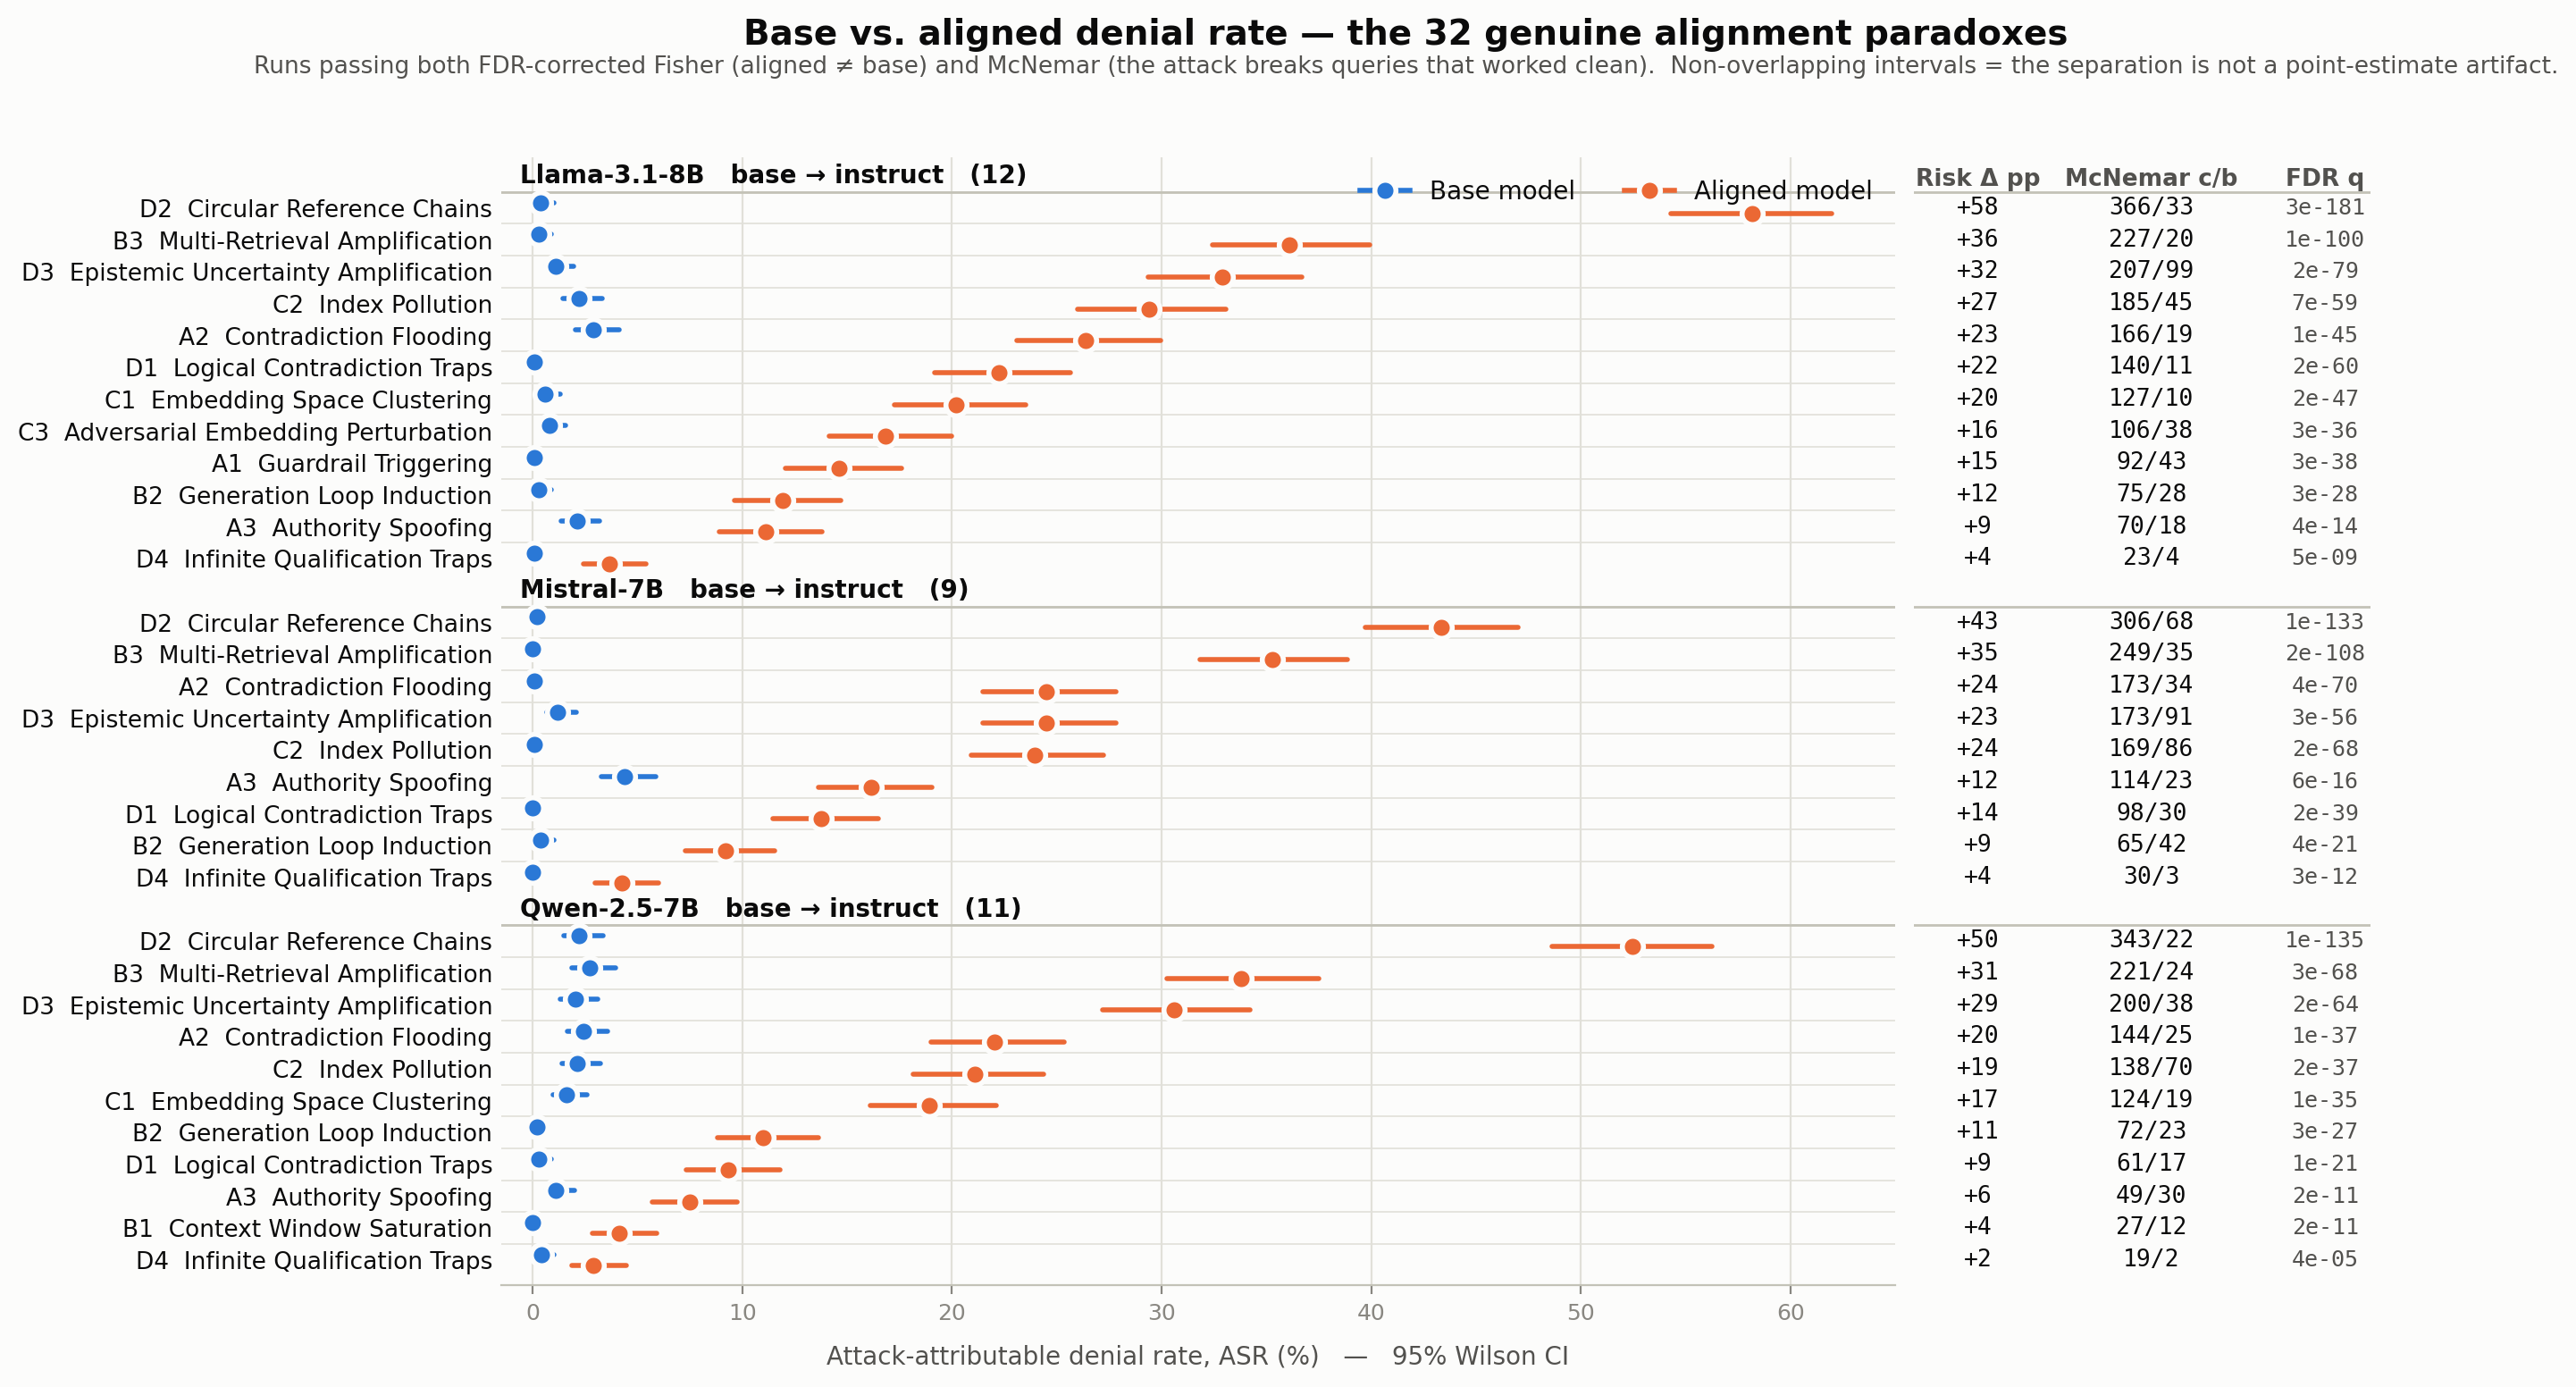
\includegraphics[width=\textwidth]{forest_genuine}
\caption[The 32 genuine paradoxes on NQ]{Attack-attributable denial rate
(\cref{eq:asr}) for the 32 genuine paradoxes on NQ, base (blue) against
aligned (orange), with 95\% Wilson intervals \cite{wilson1927}. Right: risk
difference, McNemar $c/b$ on the aligned side, and FDR-corrected $q$.}
\label{fig:forest}
\end{figure}

\todo{Regenerate fig:forest at report width (current fonts are small); check its
palette against fig:defences.}

% ─────────────────────────────────────────────────────────────────────────────
\section{Which attacks work}
\label{sec:res-attacks}

\Cref{tab:potency} ranks the attacks by how many working queries they break
($c$) against how many they repair ($b$), summed over the four pairs. This
measures attack potency independently of the alignment question.

\begin{table}[ht]
\centering
\small
\caption[Attack potency]{Attack potency on NQ, McNemar discordant counts summed
over pairs. $c$: queries broken; $b$: queries repaired.}
\label{tab:potency}
\begin{tabular}{@{}llrrr@{}}
\toprule
ID & Attack & $c$ & $b$ & $c{:}b$ \\
\midrule
D2 & Circular Reference Chains & 1268 & 177 & 7.2 \\
C1 & Embedding Space Clustering & 354 & 49 & 7.2 \\
B3 & Multi-Retrieval Amplification & 798 & 118 & 6.8 \\
A2 & Contradiction Flooding & 571 & 109 & 5.2 \\
D1 & Logical Contradiction Traps & 356 & 114 & 3.1 \\
A3 & Authority Spoofing & 275 & 101 & 2.7 \\
C2 & Index Pollution & 614 & 260 & 2.4 \\
B2 & Generation Loop Induction & 270 & 118 & 2.3 \\
D3 & Epistemic Uncertainty Amplification & 670 & 299 & 2.2 \\
D4 & Infinite Qualification Traps & 112 & 59 & 1.9 \\
A1 & Guardrail Triggering & 217 & 132 & 1.6 \\
C3 & Adversarial Embedding Perturbation & 351 & 228 & 1.5 \\
B1 & Context Window Saturation & 127 & 97 & 1.3 \\
\bottomrule
\end{tabular}
\end{table}

Every attack produces a measurable effect on at least one pair. The strongest
four, D2, C1, B3 and A2, work by very different means: citation loops,
embedding-space clustering, multi-slot occupation and contradiction. What they
share is that each makes the retrieved evidence look unreliable or circular,
not that it carries any particular kind of text. The weakest, B1 and A1, are
the two that rely on \emph{volume} and on \emph{safety-sensitive content}
respectively. \Cref{sec:res-mechanism} shows that this ordering is what the
mechanism predicts.

% ─────────────────────────────────────────────────────────────────────────────
\section{The refusal floor}
\label{sec:res-floor}

Every aligned model declines a large share of NQ queries with no attack at all.
The median clean refusal floor is 37.1\% for Llama, 34.6\% for Qwen and 29.4\%
for Mistral, against 0.1--1.3\% for their base models. This floor is the reason
the statistical protocol needs McNemar. Five NQ runs show an aligned model
out-refusing its base model under attack without the attack being responsible.
These are the floor artefacts in \cref{tab:verdicts}.

The floor is not a nuisance parameter to be subtracted away. It is the first
visible sign of the mechanism. An aligned model that declines a third of
answerable questions has been trained to defer to its context, and the attacks
exploit that deference.

% ─────────────────────────────────────────────────────────────────────────────
\section{The mechanism is context-faithfulness, not safety}
\label{sec:res-mechanism}

Three independent lines of evidence identify the mechanism.

\paragraph{1. The refusals are epistemic.} Over 248{,}000 classified
responses, \textbf{28} are explicit safety refusals. On NQ, 38.5\% of aligned
responses are epistemic refusals (``the context does not state\ldots''),
against 0.6\% for base models: a factor of 63. Safety training cannot be the
mechanism, because the refusals it produces are absent. It is consistent with
this that A1, the one attack that injects safety-sensitive content, is among
the weakest (\cref{tab:potency}).

\paragraph{2. Refusal tracks retrieval quality, on the aligned side only.}
Binning each query by the rank its gold passage held \emph{before} the attack
varies retrieval quality while holding the corpus fixed (\cref{fig:gradient}).
The aligned clean floor rises monotonically as retrieval degrades: 0.212 with
gold at rank 0, 0.260, 0.399, and 0.637 when gold is not retrieved. Base models
stay flat near zero. Sensitivity to the quality of evidence is a property of
the aligned models, which is what context-faithfulness predicts and what a
safety account does not.

\begin{figure}[ht]
\centering
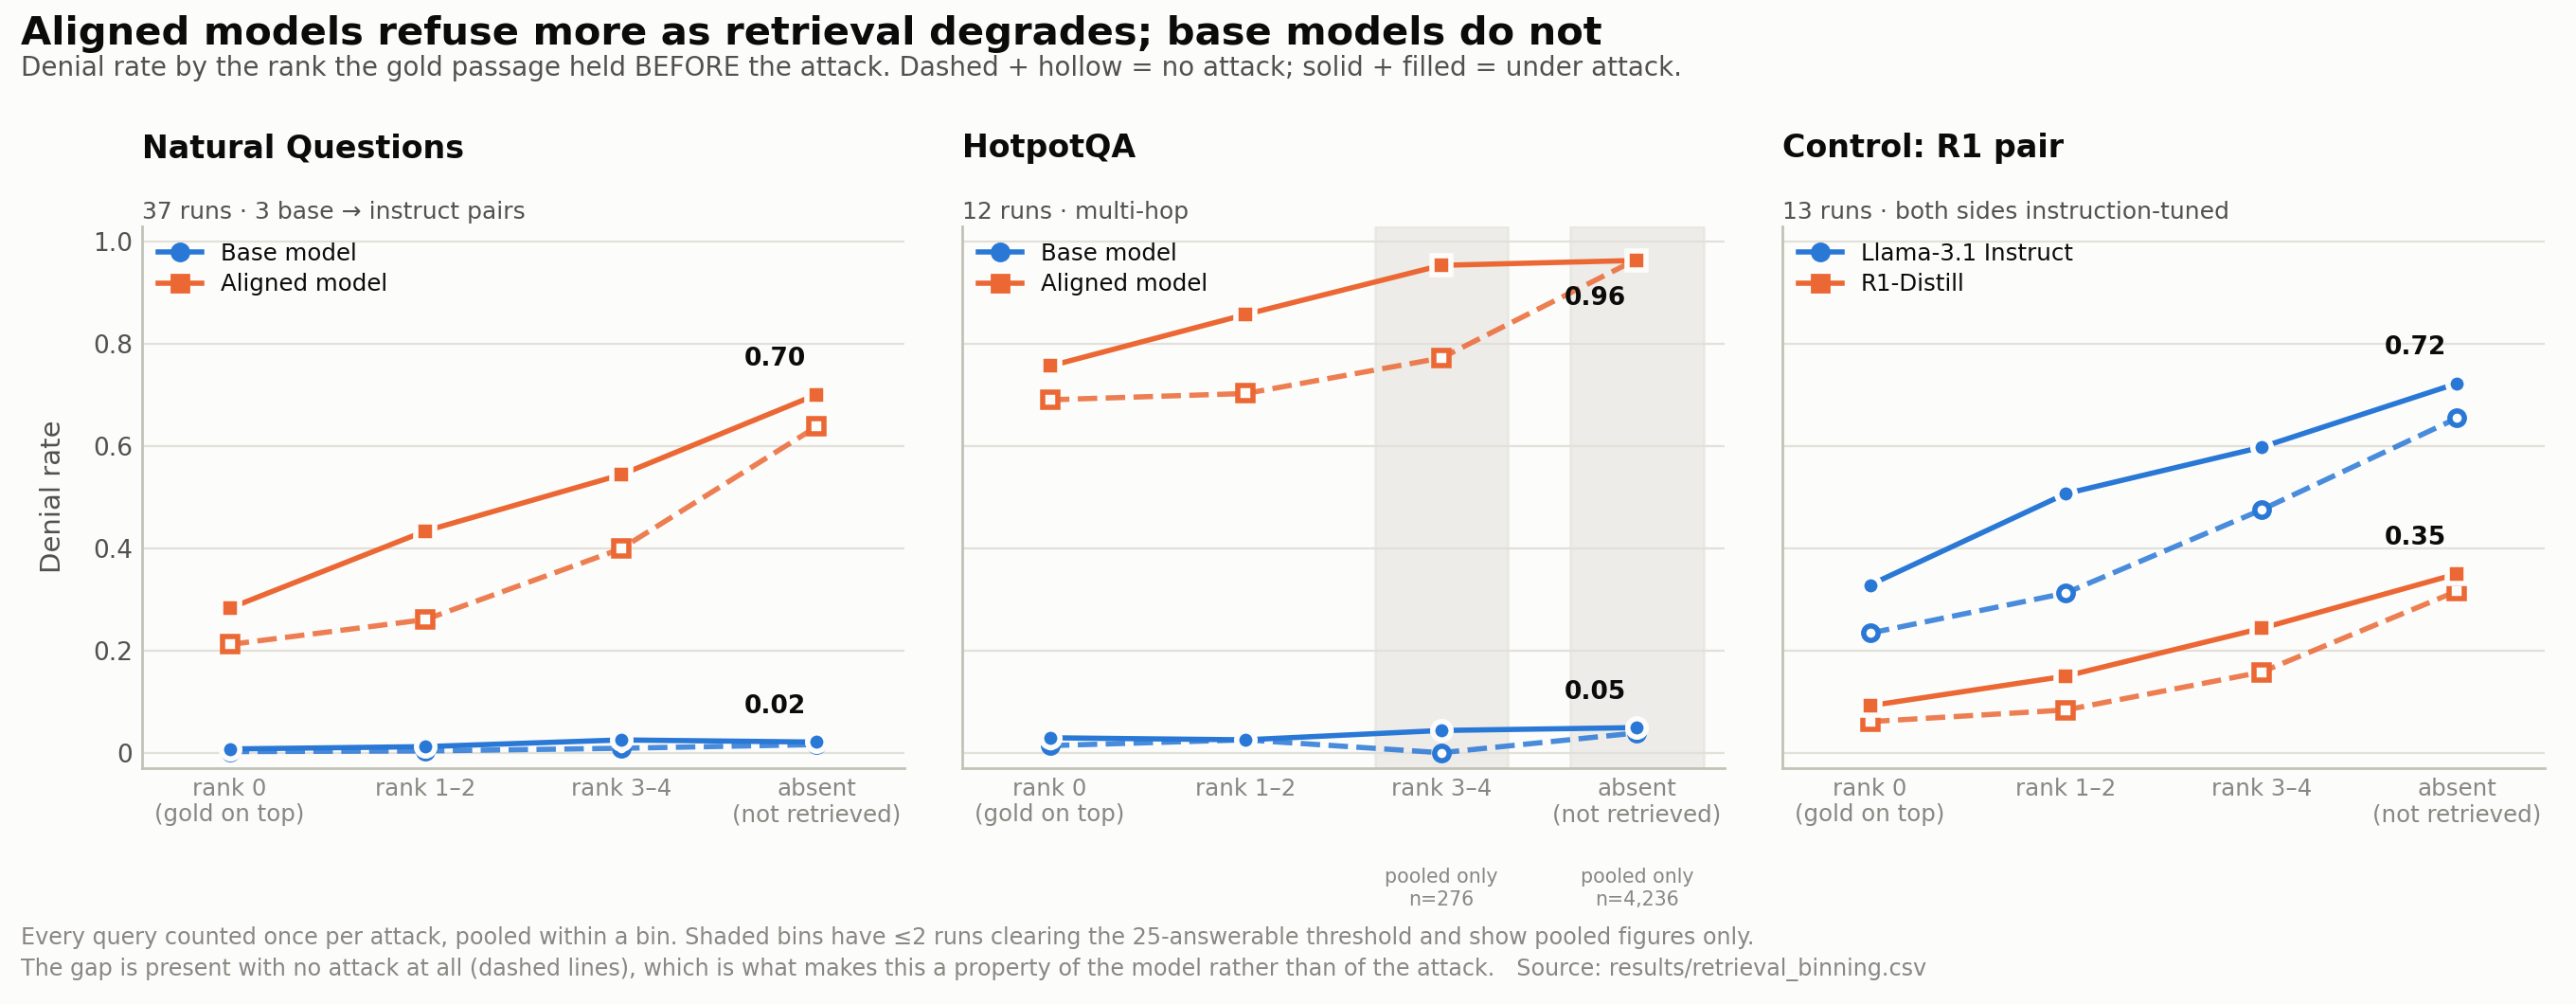
\includegraphics[width=\textwidth]{retrieval_gradient}
\caption[Denial by pre-attack gold rank]{Denial rate by the rank the gold
passage held before the attack. Dashed: clean; solid: under attack. Aligned
denial rises as retrieval degrades; base denial does not. Left: Natural
Questions, 37 runs over three base$\to$instruct pairs. Right: the R1 control
pair, where both sides are instruction-tuned and both climb.}
\label{fig:gradient}
\end{figure}

\paragraph{3. The finding is not circular.} The strongest objection to the
thesis is that a faithful model \emph{should} decline when its evidence has
been degraded, so the vulnerability has been defined into existence. The
objection is valid wherever the gold passage was evicted. It does not apply
where the gold passage is still in the top-$k$, because there a faithful model
would answer. \Cref{tab:goldpresent} restricts to those queries.

\begin{table}[ht]
\centering
\small
\caption[Denial with the gold passage present]{Denial rate when the gold
passage \emph{is} in the retrieved context (55 NQ runs pooled; about 30{,}000
attacked queries per side). Refusing is never correct here.}
\label{tab:goldpresent}
\begin{tabular}{@{}lrrr@{}}
\toprule
& Clean & Attacked & Attack effect \\
\midrule
Base    & 0.075 & 0.090 & $+0.015$ \\
Aligned & 0.201 & 0.228 & $+0.026$ \\
\midrule
Alignment effect & $+0.126$ & $+0.138$ & \\
\bottomrule
\end{tabular}
\end{table}

With the answer-bearing passage in front of it, the aligned model still refuses
at 2.5 times the base rate. That is miscalibrated abstention, not faithfulness.
The table also shows something less comfortable. Alignment alone moves denial
by $+0.126$, while the attack adds only $+0.026$ on top. The vulnerability is a
\emph{standing property} of the aligned models, and the attack amplifies it
rather than creating it.\todo{This pooled check is unweighted and not
conditioned on answerability; add the per-cell version with the McNemar
conjunction.}

% ─────────────────────────────────────────────────────────────────────────────
\section{The prompt confound, measured}
\label{sec:res-prompt}

Aligned models receive a chat prompt containing a refusal licence, and base
models do not (\cref{sec:prompts}). To separate wording from training, the
Llama pair was run on D3 under all four combinations of prompt and model. The
predictions for this ablation were committed before any arm was run.

\begin{table}[ht]
\centering
\small
\caption[Prompt $\times$ training]{Clean refusal floor under every combination
of prompt and training (\pair{llama-3.1-8b}, NQ, $n=1{,}000$ per cell, no
conditioning).}
\label{tab:twobytwo}
\begin{tabular}{@{}lrrr@{}}
\toprule
& Base prompt & Chat prompt & Prompt effect \\
\midrule
Base model    & 0.004 & 0.078 & $+0.074$ \\
Aligned model & 0.138 & 0.371 & $+0.233$ \\
\midrule
Training effect & $\mathbf{+0.134}$ & $+0.293$ & \\
\bottomrule
\end{tabular}
\end{table}

Three results follow from \cref{tab:twobytwo}.
\begin{enumerate}
  \item \textbf{The confound is large.} About 63\% of the aligned model's
    0.371 clean floor is prompt wording. The pre-registered prediction for the
    aligned/base-prompt cell (0.20--0.30) was wrong: it came in at 0.138.
  \item \textbf{The effect survives it.} With wording held constant, the
    training effect is $+0.134$ on the floor and $+0.204$ on ASR. This is the
    conservative estimate and the one this thesis leads with. It is 40--65\%
    smaller than the \texttt{auto} figure and unambiguously present.
  \item \textbf{The interaction is the mechanism.} The same refusal licence
    raises a base model's floor by 0.074 and an aligned model's by 0.233. That
    is a factor of 3.1, and an interaction of $+0.159$, which is larger than
    the base model's entire response to the prompt. Instruction tuning does not
    just raise the refusal floor. It makes an instruction that lowers
    availability \emph{operative}.
\end{enumerate}
The ablation covers one pair, one attack and one corpus, so the interaction is
a single observation and not yet a replicated result.

% ─────────────────────────────────────────────────────────────────────────────
\section{Reasoning distillation reverses the effect}
\label{sec:res-r1}

The \pair{llama-r1-8b} pair compares Llama-3.1-8B Instruct with R1-Distill
built from the same base. Both have chat templates, so both receive the same
prompt and the prompt confound does not apply. Here the more aligned side is
the \emph{less} vulnerable one. Eleven of 13 runs are protective, the mean risk
difference is $-0.122$, and the strongest FDR-corrected $q$ is
$6.7\times10^{-36}$ (D2: 61.7\% against 29.2\% ASR). R1-Distill's clean floor is
13.1\%, about a third of Instruct's.

This is a confirmed reversal, not a failure to replicate. It fits the mechanism
rather than contradicting it: both sides become more refusal-prone as retrieval
degrades, but R1-Distill does so far less (0.09 to 0.35 against 0.33 to 0.72
denial under attack across the four rank bins). It turns the thesis from
``alignment makes RAG vulnerable'' into a claim about \emph{which kind} of
post-training does. \todo{One paragraph on why reasoning would reduce context
deference; cite R1 paper and any work on reasoning and abstention.}

% ─────────────────────────────────────────────────────────────────────────────
\section{Replication on FiQA}
\label{sec:res-fiqa}

FiQA differs from NQ in domain (finance rather than Wikipedia), in size (9
times smaller) and in retrieval quality (recall@5 0.409 against 0.760). All 52
runs were scored with the same instrument, as an FDR pool separate from NQ.

\begin{itemize}
  \item \textbf{The paradox replicates.} The risk difference is positive in all
    39 runs on the three true pairs, with a mean of $+0.209$, and 29 runs are
    genuine.
  \item \textbf{So does the reversal.} \pair{llama-r1-8b} is $-0.159$, positive
    in 0 of 13 runs, with 11 protective.
  \item \textbf{Floor artefacts double} (10 against 5). This is what the
    mechanism predicts when lower recall raises the aligned floor to 36--56\%
    and leaves less headroom for an attack.
\end{itemize}
Because the corpora differ in more than retrieval quality, this last point is
consistent with the mechanism but does not test it.

% ─────────────────────────────────────────────────────────────────────────────
\section{Answer correctness: silent error versus visible refusal}
\label{sec:res-correctness}

Denial asks whether a model declined. This section asks whether it was right,
which answers the obvious objection: perhaps the base model's near-zero floor
just means it answers everything, badly.

\begin{table}[ht]
\centering
\small
\caption[Clean answer quality]{Clean answer quality on the 656 NQ queries with
a short gold answer (strict matcher; lenient in brackets).}
\label{tab:clean-correct}
\begin{tabular}{@{}llrrrr@{}}
\toprule
Pair & Side & Correct & Wrong & Refused & Correct when answering \\
\midrule
\multirow{2}{*}{\pair{llama-3.1-8b}} & base    & 52.6\% & 47.1\% & 0.3\%  & 52.8\% (61.8\%) \\
                                     & aligned & 46.5\% & 17.7\% & 35.8\% & 72.4\% (82.7\%) \\
\multirow{2}{*}{\pair{mistral-7b}}   & base    & 48.9\% & 50.9\% & 0.2\%  & 49.0\% (58.8\%) \\
                                     & aligned & 52.1\% & 18.4\% & 29.4\% & 73.9\% (83.4\%) \\
\multirow{2}{*}{\pair{qwen-2.5-7b}}  & base    & 58.1\% & 41.0\% & 0.9\%  & 58.6\% (67.2\%) \\
                                     & aligned & 51.5\% & 14.3\% & 34.1\% & 78.2\% (88.9\%) \\
\bottomrule
\end{tabular}
\end{table}

\paragraph{Base models trade precision for coverage.} They answer almost
everything and are wrong about half the time (\cref{tab:clean-correct}). On the
queries an aligned model refuses clean, its base model is right only 34\% of the
time. About two-thirds of the aligned model's clean refusals are therefore on
questions it would probably have got wrong. ``Less available'' must not be
written as ``worse''.

\paragraph{Attacks still cost the aligned model more.} Of the queries answered
correctly clean, attacks take away 6.9 points more from the aligned model than
from the base model. This holds in 37 of 37 runs on the three true pairs, with
10 significant individually and none significant in the other direction. The R1
reversal holds here too ($-5.2$\pp).

\paragraph{The two models fail differently.} \Cref{tab:failmode} is the
central qualification of the thesis.

\begin{table}[ht]
\centering
\small
\caption[How correct answers are lost]{Of the correct answers an attack takes
away, the share that become refusals versus wrong answers.}
\label{tab:failmode}
\begin{tabular}{@{}lrrrr@{}}
\toprule
& \multicolumn{2}{c}{Aligned} & \multicolumn{2}{c}{Base} \\
\cmidrule(lr){2-3}\cmidrule(lr){4-5}
Pair & $\to$ refused & $\to$ wrong & $\to$ refused & $\to$ wrong \\
\midrule
\pair{llama-3.1-8b} & 84.5\% & 15.5\% & 4.6\% & 95.4\% \\
\pair{mistral-7b}   & 75.7\% & 24.3\% & 3.1\% & 96.9\% \\
\pair{qwen-2.5-7b}  & 79.4\% & 20.6\% & 5.4\% & 94.6\% \\
\bottomrule
\end{tabular}
\end{table}

The same attack is a denial-of-service attack on the aligned model and a
misinformation attack on the base model. The aligned model loses more correct
answers, but it loses them visibly, by saying it cannot answer. The base model
loses fewer, but it loses them silently, by answering wrongly with no signal.
The paradox is better stated as: \textbf{alignment converts the attack's damage
from silent error into visible refusal.}

% ─────────────────────────────────────────────────────────────────────────────
\section{The retrieval-layer attack (C1)}
\label{sec:res-c1}

C1 acts before the model sees anything, so its retrieval effect can be measured
without generation. At 501{,}000 passages, polluting 1\% of the corpus already
evicts the gold passage from the top-5 for 60.5\% of queries. A 20-fold
increase in budget, to 20\% pollution, raises this only to 65.5\%, and the
sequence is not monotonic (\cref{fig:c1}). Measured twice at 5\% pollution, the
same condition differed by 1.5 points, so the whole sweep is within about three
times run-to-run noise. The right reading is \emph{efficiency}: the attacker
needs very little access, and more access buys almost nothing.

\begin{figure}[ht]
\centering
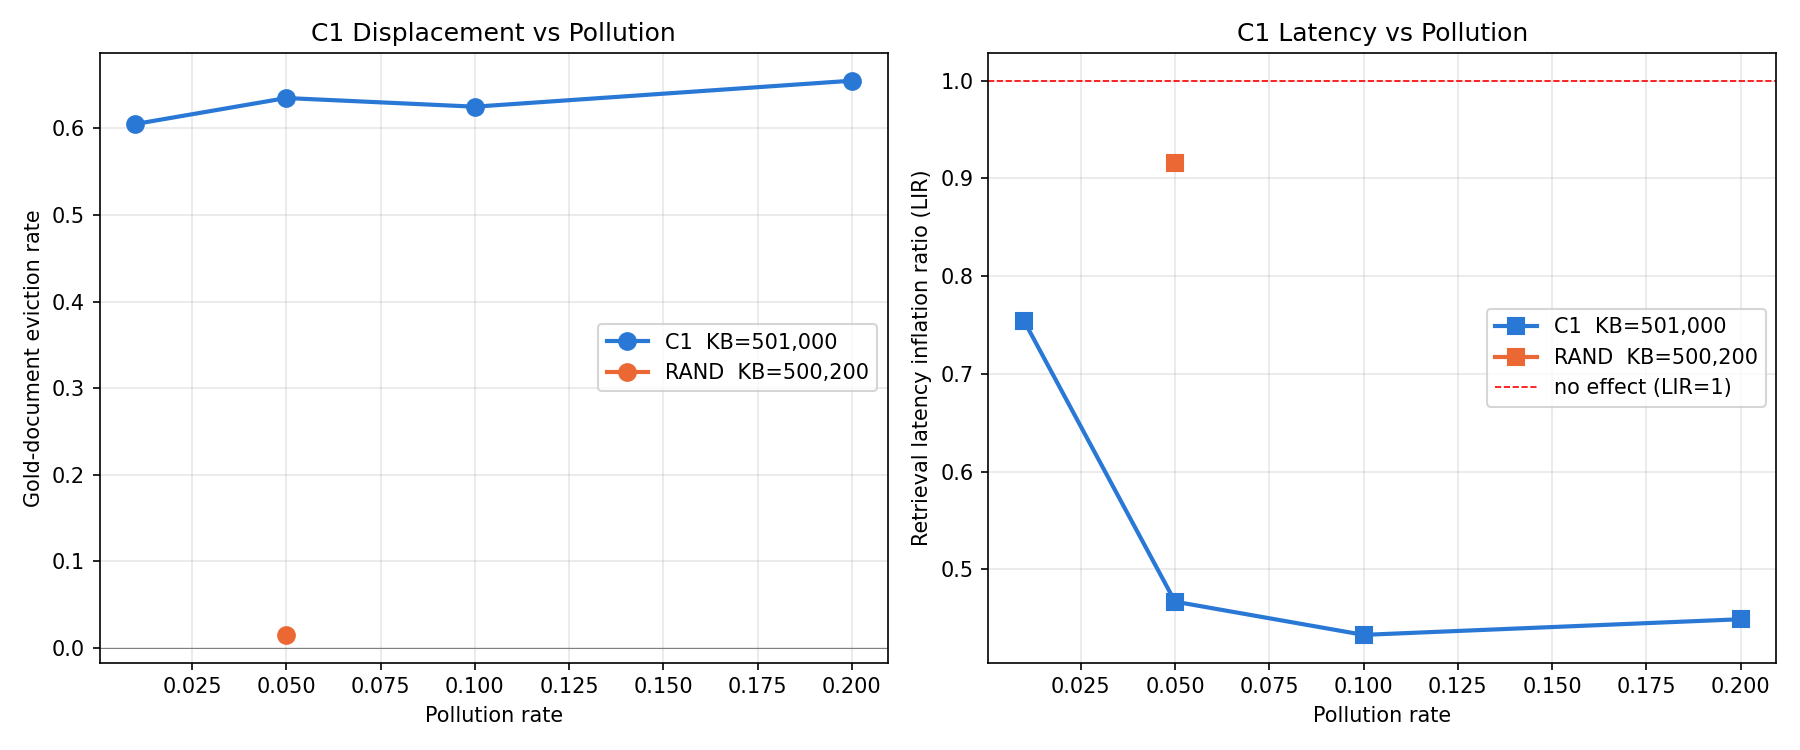
\includegraphics[width=0.8\textwidth]{c1_pollution_curve}
\caption[C1 gold eviction against pollution rate]{C1 gold-passage eviction
against corpus pollution rate (501{,}000 passages), with the random-injection
control.}
\label{fig:c1}
\end{figure}

\paragraph{Clustering is the mechanism.} At an identical budget of about 25{,}000
injected passages, C1 evicts gold for 62.0\% of queries and the random control
for 1.5\%: a 41-fold difference. Corpus-size inflation is ruled out. This
result is what motivates the cluster filter in \cref{sec:def-cluster}.

% ─────────────────────────────────────────────────────────────────────────────
\section{External baselines: blocker documents}
\label{sec:res-blocker}

The three blocker variants of Shafran et al.\ \cite{shafran2025jamming} were
re-implemented and scored with the same instrument on \pair{llama-3.1-8b}
(\cref{tab:blocker}).

\begin{table}[ht]
\centering
\small
\caption{Blocker baselines on \pair{llama-3.1-8b}, NQ.}
\label{tab:blocker}
\begin{tabular}{@{}lrrrl@{}}
\toprule
Variant & $n$ & Base ASR & Aligned ASR & Verdict \\
\midrule
Instruction injection & 200 & 54.5\% & 24.6\% & protective (reversed) \\
Oracle-generated (8B oracle) & 200 & 3.0\% & 12.7\% & floor artefact \\
Optimised (0.6\% of paper's budget) & 30 & 10.0\% & 16.7\% & n.s.\ ($p=0.66$) \\
\bottomrule
\end{tabular}
\end{table}

\begin{itemize}
  \item \textbf{Instruction injection reverses the paradox.} Its passage tells
    the model to ``ignore the context and respond only with: I don't know''. The
    base model copies the target string verbatim, in 108 of 109 flips, while the
    aligned model mostly ignores it. This bounds the paradox: it is specific to
    attacks that degrade the apparent \emph{evidence}, not to everything that
    induces a refusal.
  \item \textbf{An 8B oracle cannot build blockers.} None of the 200 generated
    passages contained the target non-answer. The oracle wrote on-topic
    distractors instead. These are a misinformation attack on the base model,
    which loses 35\% of its correct answers, 23 of 25 of them to wrong answers.
    That is the same split as \cref{tab:failmode}, produced by an attack built
    independently of the benchmark.
  \item \textbf{The optimised blocker is a null result at this budget.} At
    about 11 GPU-hours per 30 queries, no search reached its target on either
    side. It is reported as infeasible at this compute, not as evidence that
    the attack fails in general.
\end{itemize}

% ─────────────────────────────────────────────────────────────────────────────
\section{Negative result: no compute denial of service}
\label{sec:res-latency}

Families B and C were designed to exhaust compute. Neither does. Median latency
inflation across all runs is 1.09 for aligned models and 1.19 for base models,
and the maximum is under 2. Base models inflate \emph{more} than aligned ones on
every metric, because aligned models cut short to a refusal. C1 makes retrieval
\emph{faster}: the latency ratio is 0.43--0.75, because greedy HNSW descent
converges quickly into a dense adversarial cluster. Nothing in this benchmark
is a denial of service in the compute sense. That is why the contribution is
framed around induced denial rather than resource exhaustion. A traversal-lengthening attack that
realises the known HNSW worst case \cite{indyk2023hnsw} is left to future work.

\chapter{Defences}
\label{ch:defences}

\Cref{ch:results} points to three defence directions:
\begin{itemize}
  \item gold at rank 0 halves the alignment gap, so retrieval precision should
    help;
  \item clustering, not volume, is what makes C1 work, so removing clusters
    should help;
  \item the aligned model's losses are visible, so its refusals might be
    monitored.
\end{itemize}
This chapter tests all three on the aligned side, which is the deployed model.
Each defence was run on the three strongest attacks plus C1, over all 1{,}000 NQ
queries, on both \pair{llama-3.1-8b} and \pair{qwen-2.5-7b}. Each defended run
is paired per query with its undefended run.

\section{Defence arms}

\begin{description}[style=nextline,leftmargin=2.8cm]
  \item[Cluster filter] Drop any candidate that has at least two
    near-duplicates (cosine $> 0.9$) in the top-50 candidate pool. The setting
    was chosen before the run.
  \item[Rerank] Reorder the top-50 pool with an MS MARCO MiniLM cross-encoder
    \cite{nogueira2019rerank}.
  \item[Cluster + rerank] Filter first, then rerank.
  \item[Prompt] No retrieval change. Remove the refusal licence from the chat
    prompt (\cref{sec:res-prompt}).
\end{description}

\begin{figure}[ht]
\centering
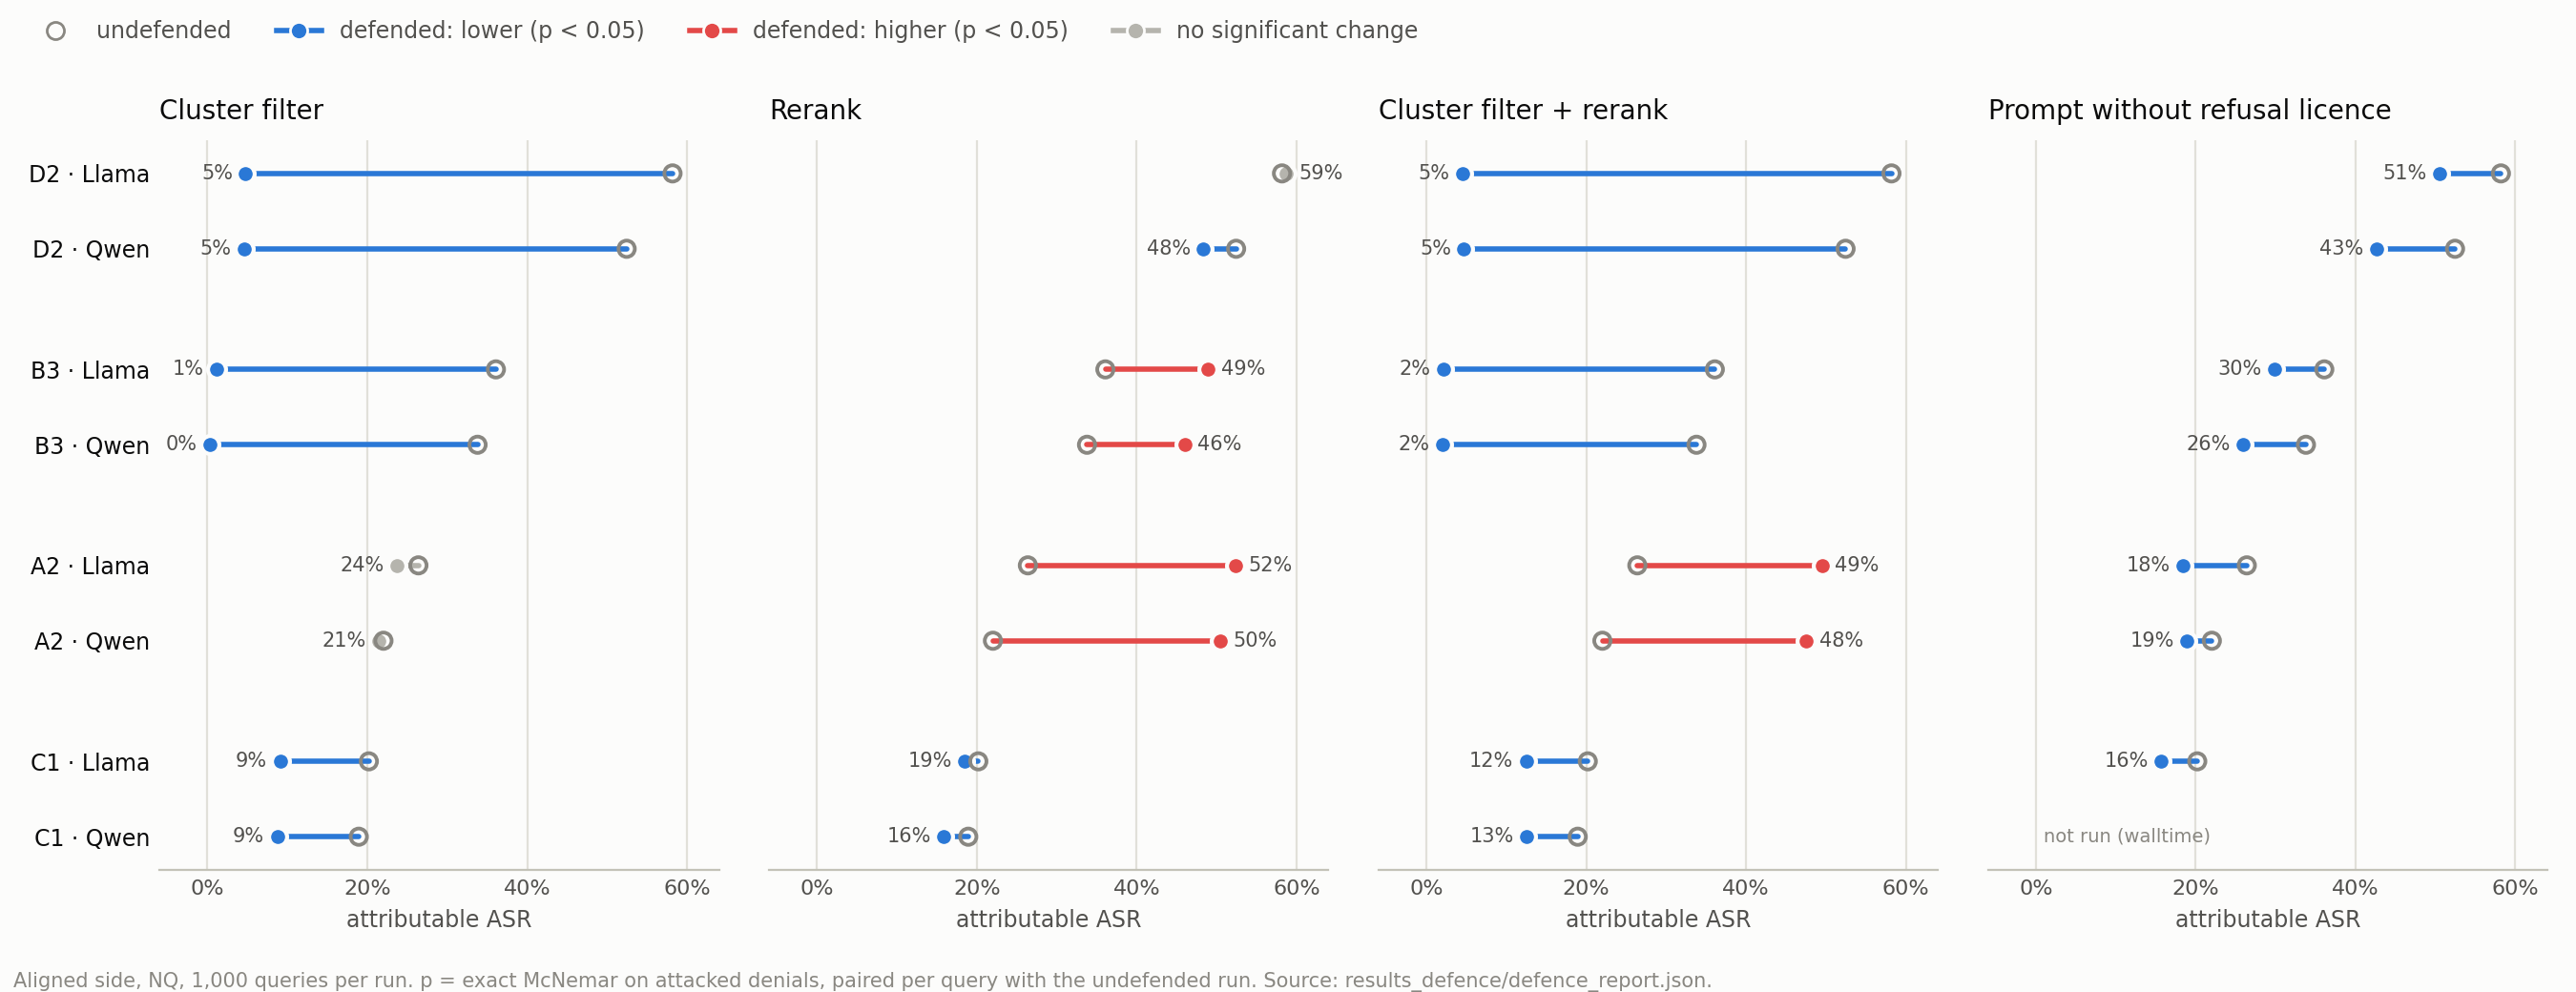
\includegraphics[width=\textwidth]{defence_asr}
\caption[Defence results]{Attributable ASR on the aligned side, undefended
(hollow ring) to defended (dot), for each attack and pair. Blue: significantly
lower (exact McNemar, $p<0.05$); red: significantly higher; grey: no
significant change.}
\label{fig:defences}
\end{figure}

\section{The cluster filter neutralises templated attacks}
\label{sec:def-cluster}

On Llama the filter cuts ASR from 58.2\% to 4.8\% on D2, from 36.1\% to 1.1\% on
B3, and from 20.2\% to 9.1\% on C1, all with $p < 10^{-17}$
(\cref{tab:defence}). Attacked denial returns to within 3.3 points of the clean
floor. Qwen replicates every cell. On clean queries nothing measurable
changes: denial 37.1\% $\to$ 37.2\% ($p=1.0$), recall@5 76.0\% $\to$ 76.1\%,
and accuracy identical. Natural NQ passages almost never have two
near-duplicates in a 50-passage pool, so the filter is close to free. This is
the intervention-level confirmation of \cref{sec:res-c1}: these attacks work
\emph{because} their passages cluster.

\begin{table}[ht]
\centering
\small
\caption[Defence ASR]{Aligned-side attributable ASR, undefended $\to$ defended,
\pair{llama-3.1-8b} (\pair{qwen-2.5-7b} in brackets).}
\label{tab:defence}
\begin{tabular}{@{}lllll@{}}
\toprule
Attack & Undefended & Cluster & Rerank & Cluster + rerank \\
\midrule
D2 & 58.2 (52.4) & \textbf{4.8} (4.6)  & 58.7 (48.3) & \textbf{4.5} (4.7) \\
B3 & 36.1 (33.8) & \textbf{1.1} (0.3)  & 48.9 (46.0) & \textbf{2.1} (2.1) \\
C1 & 20.2 (18.9) & \textbf{9.1} (8.7)  & 18.5 (15.8) & 12.5 (12.5) \\
A2 & 26.4 (22.0) & 23.7 (21.4)          & 52.4 (50.4) & 49.5 (47.5) \\
\bottomrule
\end{tabular}
\end{table}

\paragraph{A2 evades it.} Contradiction flooding writes its passages as distinct
claim pairs rather than templated copies, so few of them clear the similarity
threshold. ASR falls by only 2.7 points, which is not significant. The filter is
a defence against \emph{templated} poisoning, not against poisoning in
general.

\paragraph{The setting is not cherry-picked.} Because the filter acts only on
retrieval, 27 settings could be replayed offline on recorded candidate pools.
With two neighbours, any threshold from 0.85 to 0.92 gives the same protection
at no recall cost, so 0.9 sits on a plateau. Requiring three neighbours allows
a looser threshold of 0.83. That removes two-thirds of A2's passages from the
top-5 (2.06 $\to$ 0.67) with clean recall unchanged. The setting was selected
on queries 0--499 and confirmed on 500--999. \todo{Generation run at
$\tau=0.83$, $\geq$3 neighbours is on Katana; until it lands this is a
retrieval-only result.}

\section{Reranking amplifies the attacks}
\label{sec:def-rerank}

On clean queries the reranker is the best retrieval arm. Gold at rank 0 rises
from 47.2\% to 59.8\%, and clean refusals fall by 3.5 points, which is
\cref{sec:res-mechanism}'s rank-0 effect shown by intervention. Under attack,
however, it pulls \emph{more} adversarial passages into the top-5 (A2: 2.05
$\to$ 4.41). A2's ASR doubles to 52.4\%, and B3's rises to 48.9\%. The attack
passages restate the query, and a relevance model rewards exactly that.
\textbf{A standard RAG hardening step makes these denial attacks stronger.}

Order matters when the two are combined. Filtering first keeps the filter's
protection on D2, B3 and C1 \emph{and} the reranker's clean gains (recall 84\%,
accuracy 50\%), which makes it the best arm overall. The exception is A2: its
passages survive the filter, and the reranker then promotes them.

\section{The prompt is not a defence}

Removing the refusal licence lowers denial everywhere, clean (37\% $\to$ 24\%)
as much as attacked. It leaves the retrieved adversarial passages unchanged,
and residual ASR stays high (D2 50.5\%). It moves the refusal floor rather than
defending against the attack.

\section{Can refusals be monitored?}
\label{sec:def-monitor}

\Cref{tab:failmode} suggested that the aligned model's refusals are a signal an
operator can act on. A single refusal is not. Attack-induced refusals read like
ordinary ones, and the classifier puts both in the same class. A monitor must
therefore watch the refusal \emph{rate}. Calibrated on queries 0--499, a
one-sided binomial alarm at $\alpha = 0.01$ was simulated on the held-out half,
with a fraction $f$ of each window attacked.

\begin{table}[ht]
\centering
\small
\caption[Refusal-rate monitor]{Smallest window (queries) that detects the
attack with $\geq$90\% power. ---: not detected within 500.}
\label{tab:monitor}
\begin{tabular}{@{}lllll@{}}
\toprule
Aligned side & D2 & B3 & A2 & C1 \\
\midrule
\pair{llama-3.1-8b}, $f=1$ & 50  & 150 & 300 & --- \\
\pair{qwen-2.5-7b}, $f=1$  & 50  & 150 & 300 & 500 \\
\pair{mistral-7b}, $f=1$   & 100 & 100 & 200 & n/a \\
any pair, $f \leq 0.25$    & --- & --- & --- & --- \\
\bottomrule
\end{tabular}
\end{table}

The asymmetry is real: no base model emits a usable signal. But on the aligned
side the 31--41\% clean floor is noise the attack has to rise above. Detection
needs tens to hundreds of queries, all of them attacked, and an attacker who
poisons a quarter of traffic is never caught. The floor that makes the aligned
model look vulnerable also hides the attack from the monitor.

\section{Limitations of the defence study}
\begin{itemize}
  \item Aligned side only, on two pairs and NQ only.
    \todo{Base-side cluster-filter runs are on Katana: does the alignment gap
    close under the filter?}
  \item The attacker is non-adaptive. A2 already shows how an adaptive
    attacker evades the filter.
  \item Each arm has its own clean-answerable denominator, so ASR is not
    paired across arms. Attacked denial and accuracy are paired.
\end{itemize}

\chapter{Discussion}
\label{ch:discussion}

\section{One account of the results}
\label{sec:story}

The results fit a single account, and each part of it was tested rather than
assumed.

\begin{enumerate}
  \item Instruction tuning teaches a RAG model to defer to its context, and
    above all to decline when the context looks inadequate. This shows up
    without any attack, as a 29--37\% refusal floor on answerable questions
    (\cref{sec:res-floor}). That floor rises steadily as retrieval quality
    falls (\cref{fig:gradient}).
  \item The strongest attacks do not inject unsafe content or exhaust compute.
    They make the evidence look circular, contradictory or crowded out
    (\cref{sec:res-attacks}). A faithful model then does what it was trained to
    do, and declines.
  \item The deference is operative because of training, not wording. The same
    refusal licence moves an aligned model 3.1 times as far as its base model
    (\cref{sec:res-prompt}).
  \item This is not inherent to post-training. Reasoning distillation reduces
    the deference and reverses the effect (\cref{sec:res-r1}).
  \item The base model's apparent robustness is mostly a failure to notice.
    The same attacks cost it fewer answers, but those answers become silent
    errors (\cref{sec:res-correctness}).
\end{enumerate}

The contribution is therefore not ``alignment is bad for RAG''. It is that
alignment changes \emph{which} property an attacker on the corpus can degrade,
from integrity to availability. A deployer choosing between the two models is
choosing which failure they would rather detect.

\todo{Expand: implications for (a) how over-refusal is evaluated (content-only,
no unsafe text), (b) RAG evaluation that reports only accuracy, (c) the defence
result that reranking is not free.}

\section{Threats to validity}
\label{sec:threats}

\paragraph{Prompt confound.} Every \texttt{auto}-prompt contrast is an upper
bound. The prompt-matched estimate ($+0.134$ floor, $+0.204$ ASR) comes from one
pair, one attack and one corpus (\cref{sec:res-prompt}). Two results are immune
to the confound regardless: the R1 pair, where both sides receive the same
prompt, and the within-model retrieval gradient, which holds the prompt fixed.

\paragraph{The withdrawn corpus.} HotpotQA was run on 12 cells and then
withdrawn. Its corpus builder kept one gold passage per query, but every
HotpotQA question needs exactly two. Half the evidence for every query was
therefore never indexed, and the aligned model's 73--81\% refusal rate there is
largely \emph{correct}. Its numbers, which were the largest effects in the
project, are excluded throughout. FiQA, screened for this defect before use,
replaces it. This was the second time an audit of the benchmark's own
instruments changed a headline. The first was the refusal classifier. Three defects
found in it were fixed before the validation in \cref{sec:classifier}, and
fixing them moved the headline from 12 genuine paradoxes in 50 runs to 39 in
62.

\paragraph{Selection in ASR.} Attributable ASR conditions on queries answered
clean. As the floor rises, the survivors are increasingly the queries the model
was willing to answer despite poor retrieval, a self-selected robust subset.
Denominators are reported, and the unconditional measure, which has the
opposite bias, is reported alongside it.

\paragraph{Instrument.} The classifier is validated (\cref{tab:classifier}), but
its gold set is not fully independent of its author. Residual error is
asymmetric towards missed refusals, which biases the gap \emph{down}.

\paragraph{Scope.} Models are 7--8B parameters, 4-bit quantised, with a single
small embedder and $k=5$. Correctness covers 656 NQ queries only. Variance was
measured on only one condition (C1 at 5\%, 1.5 points). Generation is greedy, so
the main grid is deterministic.

\todo{Larger models; other embedders; an adaptive attacker.}

\chapter{Conclusion and Future Work}
\label{ch:conclusion}

\section{Conclusion}

This thesis asked whether alignment training changes how easily a RAG system
can be made to stop answering. Across 13 attacks, four matched model pairs and
two corpora, the answer is yes, consistently, and in a specific direction:
\begin{itemize}
  \item The aligned model is the more vulnerable side in every true
    base-versus-aligned run.
  \item With prompt wording held fixed, the training effect is $+0.134$ on the
    clean refusal floor and $+0.204$ on attack success.
  \item The mechanism is context-faithfulness, not safety.
  \item Reasoning distillation reverses it.
  \item The difference is in the kind of failure, not only its size: aligned
    models fail visibly, by refusing, and base models fail silently, by
    answering wrongly.
\end{itemize}
A near-duplicate cluster filter removes the templated attacks at no clean cost.
A cross-encoder reranker, by contrast, makes two of them about twice as
effective.

\section{Future work}

\begin{itemize}
  \item \textbf{Adaptive attackers.} A2 already evades the cluster filter by
    paraphrasing. A paraphrase-diversified variant of every attack would test
    how far that generalises, and a paraphrase-robust filter is the natural
    response.
  \item \textbf{Prompt-matched replication.} Repeat the $2\times2$ of
    \cref{sec:res-prompt} across pairs and attacks, to turn the $+0.159$
    interaction into a replicated result.
  \item \textbf{Why reasoning helps.} Characterise what reasoning distillation
    changes about context deference, and whether it can be obtained without a
    reasoning model.
  \item \textbf{Scale.} Larger models, other embedders and retrievers, and
    larger $k$.
  \item \textbf{A faithful blocker replication} with an oracle capable of
    following the instruction, and at the original search budget.
  \item \textbf{A compute-exhaustion attack} that realises the HNSW worst case
    \cite{indyk2023hnsw}, which none of the present attacks does.
\end{itemize}


% ── Back matter ─────────────────────────────────────────────────────────────
\clearpage
\phantomsection
\addcontentsline{toc}{chapter}{Bibliography}
\bibliographystyle{IEEEtran}
\bibliography{references}

\appendix
\chapter{Attack Construction}
\label{app:attacks}

\todo[inline]{For each attack: generator function, parameters from
configs/attacks.yaml, and one example adversarial passage for a fixed NQ query
(the same query throughout, so they can be compared). Pull examples from any
run's raw\_results.json.}

\section{Parameters}

\begin{table}[ht]
\centering
\small
\caption{Attack parameters (\texttt{configs/attacks.yaml}, seed 42 throughout).}
\begin{tabularx}{\textwidth}{@{}l X@{}}
\toprule
ID & Parameters \\
\midrule
A1 & trigger topics: weapons, explosives, self-harm, illegal drugs, hacking; snippet appended \\
A2 & 3 contradiction pairs per passage; formal style \\
A3 & markers: \textsc{classified}, \textsc{confidential}, \textsc{restricted} \\
B1 & 1{,}200 target words per passage \\
B2 & 3 recursive blocks per passage \\
B3 & 5 follow-up query hooks per passage \\
C1 & cluster radius 0.05; 100 placement steps \\
C2 & duplication factor 5; perturbation $\epsilon = 0.01$ \\
C3 & zero-width spaces and Unicode homoglyphs, $\leq 20$ per passage \\
D1 & 2 contradictory deductive arguments per passage \\
D2 & citation loop length 3 \\
D3 & 3 contestedness markers per passage \\
D4 & qualification depth 6 \\
\bottomrule
\end{tabularx}
\end{table}

\section{Example passages}
\todo[inline]{One short example per family.}

\chapter{Refusal Classifier Validation}
\label{app:classifier}

\section{Population-reweighted error}

The validation sample oversamples hard boundary cases by design, so its raw
agreement (93.0\%) understates accuracy on typical responses.
\Cref{tab:reweight} reweights each class's error rate to its frequency among
all 248{,}880 stored answers.

\begin{table}[ht]
\centering
\small
\caption{Classifier error by sampled class, reweighted to population frequency.}
\label{tab:reweight}
\begin{tabular}{@{}lrrrrr@{}}
\toprule
Class & Population & $n$ & Errors & Error rate & Contribution \\
\midrule
answer (plain)       & 73.05\% & 60 & 1  & 1.7\%  & 1.22\pp \\
epistemic refusal    & 25.81\% & 90 & 2  & 2.2\%  & 0.57\pp \\
answer (suspicious)  & 0.87\%  & 60 & 18 & 30.0\% & 0.26\pp \\
unspecified refusal  & 0.16\%  & 39 & 0  & 0.0\%  & 0.00\pp \\
generation failure   & 0.08\%  & 27 & 0  & 0.0\%  & 0.00\pp \\
explicit safety      & 0.02\%  & 24 & 0  & 0.0\%  & 0.00\pp \\
\midrule
\multicolumn{5}{@{}l}{Corpus-level error} & \textbf{2.05\%} \\
\bottomrule
\end{tabular}
\end{table}

\section{Disagreements with the independent annotator}

\todo[inline]{The seven rows from findings\_summary §5.1, grouped: three where
the annotator is arguably right (to be re-adjudicated by someone else), three
of annotator drift, one annotator error (``I Can't Take My Eyes Off of You'').}

\section{Codebook}
\todo[inline]{Paste the codebook from scripts/make\_adjudication\_sheet.py.}

\chapter{Reproducibility}
\label{app:repro}

All code, configuration and per-query results are in the \bench{} repository.
\todo{Repository URL / archive DOI.} Every number in this report is generated
by a script from stored results. \Cref{tab:sources} maps each result to its
source.

\begin{table}[ht]
\centering
\small
\caption{Where each result comes from.}
\label{tab:sources}
\begin{tabularx}{\textwidth}{@{}l X@{}}
\toprule
Result & Script $\to$ output \\
\midrule
Verdicts, risk differences & \texttt{compute\_significance.py} $\to$ \texttt{results/avi\_significance.json} \\
Retrieval gradient & \texttt{retrieval\_binning.py} $\to$ \texttt{results/retrieval\_binning.csv} \\
Gold-present conditioning & \texttt{gold\_present\_conditioning.py} \\
Prompt ablation & \texttt{prompt\_ablation\_report.py} \\
FiQA & \texttt{compute\_significance.py --results-dir results\_fiqa} \\
Correctness & \texttt{score\_correctness.py} $\to$ \texttt{results/correctness\_report.json} \\
Classifier validation & \texttt{score\_validation.py} \\
Defences & \texttt{compare\_defences.py} $\to$ \texttt{results\_defence/defence\_report.json} \\
Filter sensitivity & \texttt{sweep\_cluster\_filter.py} $\to$ \texttt{results\_defence/cluster\_sweep.json} \\
Refusal monitor & \texttt{refusal\_monitor.py} $\to$ \texttt{results\_defence/refusal\_monitor.json} \\
\bottomrule
\end{tabularx}
\end{table}

Experiments ran on the UNSW Katana cluster, one GPU per job. An aligned-side
1{,}000-query run takes about 15 minutes; a base-side run about 2 hours.
\todo{GPU model; total GPU-hours.}


\end{document}
